\documentclass{beamer}
\usepackage[russian]{babel}
\usetheme{metropolis}

\usepackage{amsthm}
\setbeamertemplate{theorems}[numbered]

\setbeamercolor{block title}{use=structure,fg=white,bg=gray!75!black}
\setbeamercolor{block body}{use=structure,fg=black,bg=gray!20!white}

\usepackage[T2A]{fontenc}
\usepackage[utf8]{inputenc}

\usepackage{hyphenat}
\usepackage{amsmath}
\usepackage{graphicx}

\AtBeginEnvironment{proof}{\renewcommand{\qedsymbol}{}}{}{}

\title{
Микроэкономика-I
}
\author{
Павел Андреянов, PhD
}

\begin{document}

\maketitle

\section{Кривая Энгеля}

\begin{frame}{Кривая Энгеля}

Если взять две кривые доход-потребление: $x^{\ast}(I), y^{\ast}(I)$, то получится параметрически заданная кривая в пространстве товаров $(x,y)$. 

Вот эта кривая и называется кривой Энгеля.

\end{frame}

\section{Кобб-Дуглас}

\begin{frame}{Кобб-Дуглас}

\begin{definition}
Полезностью \textbf{Коббп-Дугласа} называется:
$$U(x, y) = x^{\alpha} y^{1-\alpha}, \quad \alpha \in (0,1)$$  
\end{definition}

Вспомним, что монотонные преобразования полезности не меняют поведение потребителя. Тогда можно применить логарифм и получить:
$$ U(x, y) = \alpha \log x + (1-\alpha) \log y, \quad \alpha \in (0,1).$$ 
Заметим, что эта функция вогнута!!! 
\end{frame}

\begin{frame}{Кобб-Дуглас}

Выпишем Лагранжиан:
$$ \mathcal{L} = \alpha \log x + (1-\alpha) \log y - \lambda (px + qy -I).$$ 

Заметим, что я выставляю знак минус так, чтобы у множителя Лагранжа была интерпретация теневой цены выхода за бюджетное ограничение. Это нам пригодится в следующей лекции, а сейчас просто постарайтесь запомнить.
\end{frame}

\begin{frame}{Кобб-Дуглас}

Бездумно выпишем три уравнения:

$\mathcal{L}'_x = \alpha/ x - \lambda p = 0$

$\mathcal{L}'_y = (1-\alpha)/y - \lambda q = 0$

$\mathcal{L}'_{\lambda} = I - p x - qy = 0$

Легко видеть, что они эквивалентны

$\alpha - \lambda p x= 0$

$(1-\alpha) - \lambda q y= 0$

$px + qy - I = 0$

\end{frame}

\begin{frame}{Кобб-Дуглас}

Обозначим доли бюджета потраченные на $x$ и $y$ как $s_x= px$ и $s_y = qy$ соответственно, и умножим последнее уравнение на $\lambda$. 

Тогда уравнения становятся еще проще:

$\alpha = \lambda s_x$

$(1-\alpha) = \lambda s_y$

$\lambda s_x + \lambda s_y = \lambda I$

Эту систему можно уже решить в уме. 

Получается, что теневая цена равна $\lambda = 1/I$, а доли бюджета, потраченные на каждый товар, постоянны и равны $\alpha$ и $1-\alpha$.

Это интуитивно?

\end{frame}

\begin{frame}{Кобб Дуглас}

Пусть полезность имеет следующий вид:
$$U(x,y,z) = \alpha \log x + \beta \log y + \gamma \log z$$ 
а цены равны $p, q, r$ соответственно.

Спрос на каждый товар в Коббе-Дугласе описывается следующими уравнениями:
\begin{gather*}
x^{\ast} = \frac{\alpha}{\alpha + \beta + \gamma} \frac{I}{p}, \quad
y^{\ast} = \frac{\beta}{\alpha + \beta + \gamma} \frac{I}{q}, \quad
z^{\ast} = \frac{\gamma}{\alpha + \beta + \gamma} \frac{I}{r}
\end{gather*}

Такое лучше запомнить наизусть. Также постарайтесь ответить, являются ли такие товары нормальными, комплементами или субститутами.

\end{frame}

\begin{frame}{Кобб Дуглас}

Нампомним, что косвенная полезность чувствительна к монотонным преобразованиям, поэтому тут важно какая именно спецификация была изначально дана в задаче. 

Для простоты давайте считать, что это спецификация в логарифмах.

Сосчитаем логарифм спроса на первый товар:
$$\log x^{\ast} = \log \alpha - \log (\alpha + \beta + \gamma) + \log I - \log p$$
Аналогично считается логарифм спроса на другие товары. Теперь надо просто подставить их в полезность.

\end{frame}

\begin{frame}{Кобб Дуглас}

Косвенная полезность в Коббе-Дугласе (с точностью до преобразования) имеет вид
$$V(p,q,r,I) = (\alpha + \beta + \gamma) \log I - \alpha \log p - \beta \log q - \gamma \log r + C $$
Константы $C$ можно, как правило, не выписывать, так как они исчезнут при первой же попытке продифференцировать.

Эта формула нам будет очень полезна в будущем...
\end{frame}

\section{Леонтьев}

\begin{frame}{Леонтьев}

\begin{definition}
Полезностью \textbf{Леонтьева} называется:
$$U(x, y) = \min(x/a, y/b)$$  
\end{definition}

Интерпретация полезности такая, что для извлечения одной единицы полезности необходимо ровно a и b единиц потребительских товаров. Иногда такая полезность называется \textbf{совершенными комплементами}.

\end{frame}

\begin{frame}{Леонтьев}

\begin{figure}[hbt]
\centering
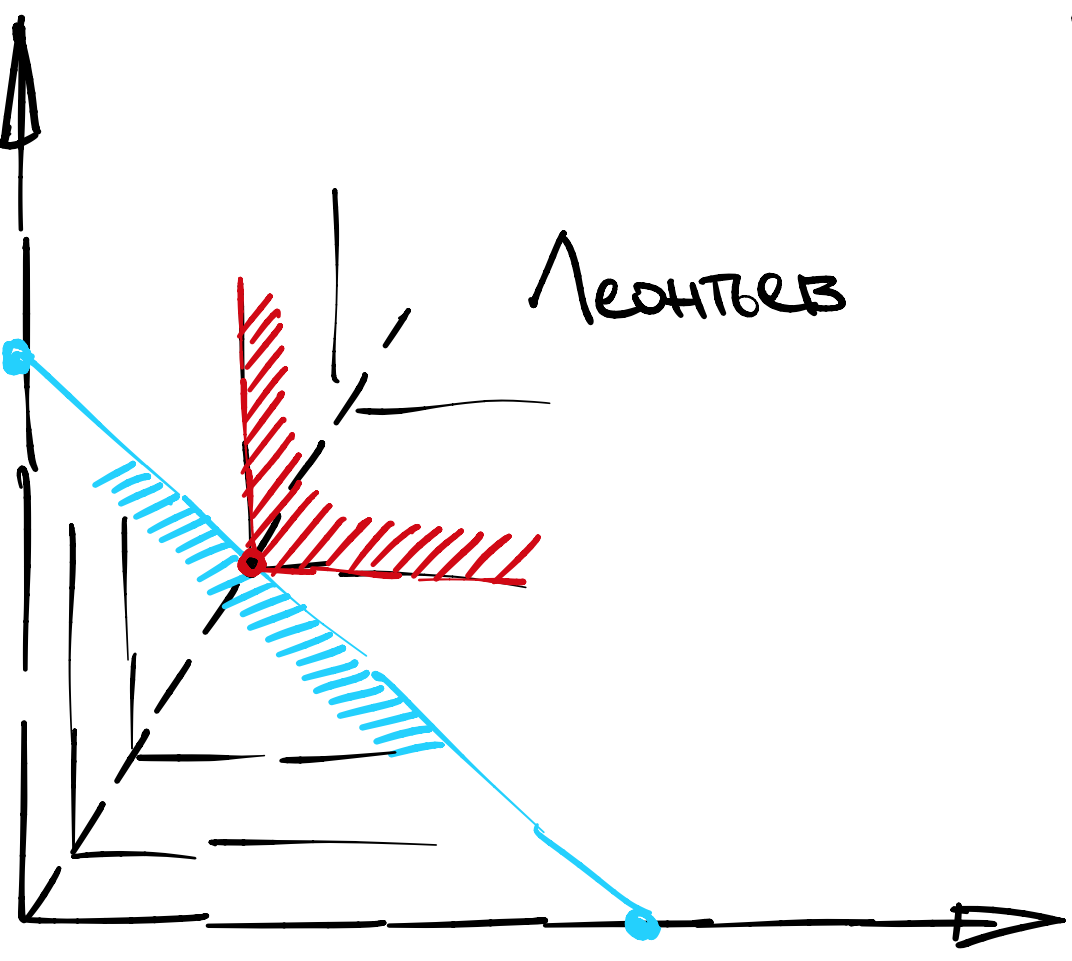
\includegraphics[width=.8 \textwidth]{leontiev}
\end{figure}

\end{frame}

\begin{frame}{Леонтьев}

Поскольку задача негладкая, то геометрический метод проще и быстрее. Решение лежит в пересечении кривой Энгеля и бюджетной линии. 

Соответственно, достаточно решить систему уравнений:
$$ px + qy = I, \quad b x = a y$$
Кривая Энгеля здесь – это множество точек, от которых отложены уголки.

\end{frame}

\begin{frame}{Леонтьев}

Пусть полезность имеет следующий вид:
$$U(x,y,z) = \min(x/a, y/b, z/c)$$ 
а цены равны $p, q, r$ соответственно. 

Спрос на каждый товар в Леонтьеве описывается следующими уравнениями:
\begin{gather*}
x^{\ast} = \frac{ap}{ap + bq + cr} \frac{I}{p}, \\
y^{\ast} = \frac{bq}{ap + bq + cr} \frac{I}{q}, \\
z^{\ast} = \frac{cr}{ap + bq + cr} \frac{I}{r}.
\end{gather*}

Все товары в функции Леонтьева являются нормальными, а также попарно являются (строго) комплементами.

\end{frame}

\begin{frame}{Леонтьев}

Заметим, что в оптимуме полезности в обоих позициях аргумента одинаковые. То есть косвенная полезность равна одновременно левому и правому аргументу.


Косвенная полезность в Леонтьеве (с точностью до преобразования) имеет вид
$$V(p,q,I) = \frac{I}{ap + bq + cr}$$

Это тоже очень полезная формула.

\end{frame}

\section{Квазилинейная}

\begin{frame}{Квазилинейная}

Пожалуй, третья самая важная полезность имеет следующий вид:

\begin{definition}
\textbf{Квазилинейной полезностью} называется:
$$U(x, y) = f(x) + k y,$$ 
где $f$ - вогнутая функция.
\end{definition}

Интерпретация последней координаты - это деньги на счету. То есть вам не обязательно тратить весь бюджет как раньше и остаток средств на счету конвертируется в утили по курсу 1:$k$.

\end{frame}

\begin{frame}{Квазилинейная}

Выпишем Лагранжиан:
$$\mathcal{L} = f(x) + k y - \lambda (px + y - I).$$ 
Легко, правда?

Обратите внимание, что цена денег равна единице.

\end{frame}

\begin{frame}{Квазилинейная}

Сейчас мы попробуем найти внутреннее решение.

$\mathcal{L}'_x = f'_x - \lambda p = 0$

$\mathcal{L}'_y = k - \lambda = 0$

$\mathcal{L}'_{\lambda} = I - p x - y= 0$

Легко видеть, что они эквивалентны

$k = \lambda$

$x = (f')^{-1}(\lambda p)$

$px + y = I$

\end{frame}

\begin{frame}{Квазилинейная}

Сейчас мы попробуем найти внутреннее решение.

$\mathcal{L}'_x = f'_x - \lambda p = 0$

$\mathcal{L}'_y = k - \lambda = 0$

$\mathcal{L}'_{\lambda} = I - p x - y= 0$

Легко видеть, что они эквивалентны

$k = \lambda$

$x = (f')^{-1}(\lambda p)$

$px + y = I$

\end{frame}

\begin{frame}{Квазилинейная}

Однако эта система не всегда имеет решение в $\mathbb{R}^2_{+}$. Легко видеть, что спрос на товар $x$ никак не зависит от бюджета, а стало быть, при достаточно маленьком бюджете спрос на товар $y$ упрется в ноль.

Мы оказались в ситуации, о которой я предупреждал. Условия первого порядка указали на точку, которая может оказаться вне допустимой области. Если это так, это значит что решение не внутреннее, а краевое. В таком случае, мы заменяем условие первого порядка  $x = (f')^{-1}(\lambda p)$ на краевое условие $y=0$ или эквивалентно $x = I/p$.

\end{frame}


\begin{frame}{Квазилинейная}

В этой задаче есть два взаимоисключающих режима: внутреннее решение и краевое решение. Но вместо перебора случаев, можно записать ответ в компактной форме, если проявить немного смекалки.

Спрос на каждый товар в квазилинейной полезности описывается следующими уравнениями:
\begin{gather*}
x^{\ast} = \min (I/p, (f')^{-1}(k p)), \\
y^{\ast} = \max (0, I-px^{\ast}).
\end{gather*}
Все товары в квазилинейной полезности являются нормальными, a деньги (переменная $y$) являются универсальным комплементом.
\end{frame}

\begin{frame}{Квазилинейная}

Поскольку в задаче два режима, скорее всего ответ будет иметь форму максимума или минимума из двух выражений. Если бы ограничения не было, решение было бы всегда внутреннее, а полезность равна 
$$f((f')^{-1}(k p)) + I - p (f')^{-1}(k p).$$

Когда ограничение активно, оно мешает нам достигнуть этой полезности и мы получаем вместо нее
$$ f(I/p) + 0.$$

\end{frame}

\section{Линейная}

\begin{frame}{Линейная}

Простая с виду, но очень неудобная на практике:

\begin{definition}
\textbf{Линейной полезностью} называется:
$$U(x, y) = x/a +y/b,$$ 
\end{definition}

интерпретируется как способность извлекать одну и туже полезность из разных источников.  Конкретно вы можете получить одну единицу полезности либо из $a$ единиц товара $x$, либо из $b$ единиц товара $y$. 

Это значит, что $x, y$ обладают высокой взаимозаменяемостью либо вообще представляют собой один и тот же товар в пачках/таре разного размера. Такая полезность еще часто называется \textbf{совершенными субститутами}.

\end{frame}

\begin{frame}{Линейная}

Решение в этой задаче не похоже на предыдущие, оно вообще всегда краевое. 

Почему так? Посмотрим внимательно на бюджетное ограничение:

$$B(x,y) = px + qy - I \leqslant 0$$ 

оно показывает, что вы можете менять товары $x, y$ по курсу $\frac{1}{p}$ к $\frac{1}{q}$. А в полезности вы можете менять товары по курсу $a$:$b$. За исключением редкого случая, когда эти курсы совпадают: 
$$ap = bq,$$ 
вам выгодно менять один товар на другой до упора.
\end{frame}

\begin{frame}{Линейная}

Осталось понять, каким будет краевое решение...

Интуитивно понятно, что вы будете тратить все на $x$, когда его вес в полезности относительно большой, а его цена относительно маленькая. То есть, когда $ap$ относительно маленький. 

Относительно чего? Конечно же, относительно $bq$.

\end{frame}

\begin{frame}{Линейная}

Осталось понять, каким будет краевое решение...

Интуитивно понятно, что вы будете тратить все на $x$, когда его вес в полезности относительно большой, а его цена относительно маленькая. То есть, когда $ap$ относительно маленький. 

Относительно чего? Конечно же, относительно $bq$.

Спрос на каждый товар описывается так: 

если $ap < bq$, то $x^{\ast} = I/p, y^{\ast} = 0$

если $ap > bq$, то $x^{\ast} = 0, y^{\ast} = I/q$

Все товары в линейной полезности нормальные и являются попарно субститутами.

\end{frame}

\begin{frame}{Линейная}

Мы знаем, что решение либо в одном углу, либо в другом. Соответственно, ответ это наибольшая из двух полезностей этих кандидатов, то есть
$$V(p,q,I) = I \cdot \max(\frac{1}{ap}, \frac{1}{bq}).$$
Пользуясь тем, что максимум коммутирует с монотонно возрастающими преобразованиями
$$ \varphi'(x) >0 \quad \Rightarrow \quad \max(\varphi(x), \varphi(x)) = \varphi(\max(x, y)$$
и с монотонно убывающими преобразованиями в некотором смысле тоже
$$ \psi'(x) < 0 \quad \Rightarrow \quad \max(\psi(x), \psi(x)) = \psi(\min(x, y)$$
можно вывести следующее красивое свойство...

\end{frame}

\begin{frame}{Линейная}

Косвенная полезность в линейной полезности (с точностью до преобразования) имеет вид
$$V(p,q,I) = I / \min(ap, bq),$$
Это тоже лучше запомнить наизусть.
\end{frame}



\section{Конец}

\end{document}